% #############################################################################
% This is Chapter 3
% !TEX root = ../main.tex
% #############################################################################
% Change the Name of the Chapter i the following line
\fancychapter{The Method of Fundamental Solutions}
% \cleardoublepage
% The following line allows to ref this chapter
\label{chap:numerical}
% #############################################################################

\section{Density and linear independence results}

The method of Fundamental Solutions is the base method to be implemented throughout this work. As a meshless method, it does not involve any kind of domain discretization (into some mesh) like in finite differences or finite elements methods. Instead, the problem is now of point placement. Since the mesh creation is one of the most computational expensive parts of the methods above, one of the main advantages of the MFS is exactly the lack of it. 

As the name implies, MFS is based on the fundamental solutions of a previously known PDE. Consider the Elliptic linear differential operator \(\mathcal{L}\) with fundamental solution \(\Phi\) such that \(\mathcal{L}\Phi(x) = \delta, \; \forall x \in \mathbb{R}^d\). Intuitively, we can consider the approximation
\[
\Tilde{u}(x) = \sum_{j=1}^{N}\alpha_j \Phi(x-y_j)
\]
to the partial differential equation with a linear boundary operator \(\mathcal{B}\)
\[
\begin{cases}
    \mathcal{L}u(x) = 0, x \in \Omega\\
    \mathcal{B}u(x) = 0, x \in \partial\Omega
\end{cases}. 
\]
By definition and using the linearity of the operator \(\mathcal{L}\), \(\tilde{u}\) satisfies the equation in \(\Omega\), and the coefficients \(\alpha_j\) can be determined by imposing the boundary conditions
\[
    \mathcal{B}\tilde{u}(x)=\sum_{j=1}^{N}\alpha_j \mathcal{B}\Phi(x-y_j)=0,
\]
where \(y_j \in \hat{\Gamma} \subset \mathbb{R}^d\setminus \overline{\Omega}\) with \(j=1,\dots,N\), are the so-called source points to be chosen. We chose them to be outside our domain since, by translation, the Fundamental Solution \(\Phi\) has a singularity at each \(y_j\) because, otherwise, it would render our approximation full of singularities inside \(\Omega\). 
\begin{remark}
    While the motivation above might seem far-fetched, one can observe that the approximation \(\Tilde{u}\) resembles a convolution between some density function \(\alpha(x)\) and the fundamental solution \(\Phi\). As we will see below, it can be proven that the fundamental solutions of the operator \(\mathcal{L}\) are dense in the functional space defined in \(\partial\Omega\) (which is enough since, as we already saw, the interior condition is satisfied by construction). For example, considering Dirichlet boundary conditions, one can use the single layer potential (which is going to be presented and studied in the next pages) that allow, through a discretization argument, to give a numerical approximation to the BVP and
    \begin{equation}\label{mfs_approx_disc}
        u(x) = \int_{\Gamma}\Phi(x-y)\varphi(y)d\sigma(y) \approx \sum_{j=1}^{N}w_j \varphi(y_j) \Phi(x-y_j) = \Tilde{u}(x), 
    \end{equation}
    where \(\varphi(y)\) is a layer density to be determined and \(y_j \in \hat{\Gamma}\) and \(w_j\) are the nodes and weights of some quadrature, respectively. Setting \(\mathcal{B} = I\) and \(\alpha_j = w_j \varphi(y_j)\), we recover the approximation given above.
\end{remark}
First, we introduce the notion of \textit{artificial boundary} (or \textit{pseudo-boundary}), which is analyzed in \cite{alves2009choice}.
\begin{definition}
    A source set \(\hat{\Gamma}\) is said to be admissible if
    \begin{enumerate}
        \item \(\hat{\Gamma} \subset \mathbb{R}^d\setminus \overline{\Omega}\) is an open set with components in each external part of \(\Omega\);
        \item \(\hat{\Gamma} = \partial \hat{\Omega}\) is the boundary of \(\hat{\Omega}\), where \(\hat{\Omega} \subset \mathbb{R}^d\setminus\overline{\Omega}\) is an open set with components in each external part of \(\Omega\). Note that the problem must be well posed in \(\hat{\Omega}\);
        \item \(\hat{\Gamma} \subset \partial \hat{\Omega}\), when \(\partial \hat{\Omega}\) is an analytical boundary set verifying (2.) and \(\hat{\Gamma}\) is open in the \(\partial \hat{\Omega}\) topology. 
    \end{enumerate}
    We denote the set of chosen source points by \(\mathcal{Y} = \{y_j \in \hat{\Gamma}: j=1,\dots,N\}\).
\end{definition}
Throughout this work, the adopted source set will always be the second option since it provides better numerical results. However, notice that the density results below still hold when considering different types of admissible source sets.

Assume that \(\mathcal{L} = -\Delta\) and \(\Phi\) is the fundamental solution of the Laplace equation. Until further notice, we are working with Dirichlet boundary conditions. Of course, the results stated below are also valid with different boundary conditions. In the appropriate functional space and given an admissible source set \(\hat{\Gamma}\), consider the approximation space
\[
    \mathcal{S}(\Gamma, \hat{\Gamma}) = \Span\{\Phi(x-y)_{|x \in \Gamma} : y \in \hat{\Gamma}\}.
\]
Some preliminary results are going to be needed in order to present the desired density proofs.
% We notice that every result below has its own counterpart if we consider \(\mathcal{L} = -(\Delta + k^2)\) and \(\Phi_k\) to be fundamental solution of the Helmholtz equation.
We start by introducing the concept of analytic continuation. For further details see \cite{narasimhan2012complex}.
\begin{definition}
    Let \(f\) be a complex valued function defined on \(\Omega \subset \mathbb{C}\). We say that \(f\) is holomorphic on \(\Omega\) if for every \(a \in \Omega\), there exists a neighborhood \(U\) of \(a\) and \((c_n)_{n \in \mathbb{N}} \subset \mathbb{C}\) such that the power series
    \[
        \sum_{n=0}^{\infty} c_n(z-a)^n
    \]
    converges to \(f(z)\) for every \(z \in U\).
\end{definition}
\begin{theorem}[Analytic continuation]\label{ana_cont}
    Let \(f\) be a holomorphic function in the connected subset \(\Omega \subset \mathbb{C}\). If there exists a non-empty \(U \subset \Omega\) such that \(f = 0\) in \(U\), then \(f = 0\) in \(\Omega\).
\end{theorem}
As seen in the above remark, the study of layer potentials plays an important role in the Method of Fundamental Solutions, which are now formalized, and some results are stated. Since this is by itself a large topic see \cite{chen2010boundary}, \cite{kress2013linear} and \cite{colton2013integral} for more details.
\begin{definition}
    Let \(\Omega\) be a bounded domain of class \(C^2\) and \(\varphi \in H^\frac{1}{2}(\Omega)\). The functions
    \[
        S\varphi(x) = \int_{\partial\Omega} \Phi(x-y)\varphi(y) d\sigma(y)
    \]
    and
    \[
        M\varphi(x) = \int_{\partial\Omega} \frac{\partial \Phi(x-y)}{\partial n}\varphi(y) d\sigma(y)
    \]
    are called the single and double layer potentials with density \(\varphi\), respectively.
\end{definition}
\begin{proposition}\label{sl_jump}
    Let \(\Omega\) be a bounded domain of class \(C^2\) and \(\varphi \in H^\frac{1}{2}(\Omega)\). Then the single layer potential is harmonic in \(\mathbb{R}^d\setminus \overline{\partial\Omega}\), continuous across \(\partial\Omega\), and for every \(x \in \partial\Omega\) we have the following jump relations for the normal derivative:
    \[
        \lim_{z \rightarrow x} \frac{\partial S\varphi}{\partial n^-}(z) = \int_{\partial\Omega} \frac{\partial\Phi(x-y)}{\partial n}\varphi(y) d\sigma(y) - \frac{1}{2}\varphi(x), \quad z \in \mathbb{R}^d \setminus \ \overline{\Omega}
    \]
    and
    \[
        \lim_{z \rightarrow x} \frac{\partial S\varphi}{\partial n^+}(z) = \int_{\partial\Omega} \frac{\partial\Phi(x-y)}{\partial n}\varphi(y) d\sigma(y) + \frac{1}{2}\varphi(x), \quad z \in \Omega.
    \]
    In particular, we have
    \[
        \varphi(x) = \frac{\partial S\varphi}{\partial n^+}(x)-\frac{\partial S\varphi}{\partial n^-}(x), \; \forall x \in \partial\Omega.
    \]
    Analogously, the double layer potential is harmonic in \(\mathbb{R}^d\setminus \overline{\partial\Omega}\), its normal derivative is continuous across \(\partial\Omega\), and for every \(x \in \partial\Omega\) we have the following jump relations:
    \[
        \lim_{z \rightarrow x} M^+\varphi(z) = \int_{\partial\Omega} \frac{\partial\Phi(x-y)}{\partial n}\varphi(y) d\sigma(y) + \frac{1}{2}\varphi(x), \quad z \in \mathbb{R}^2\setminus\overline{\Omega}
    \]
    and
    \[
        \lim_{z \rightarrow x} M^-\varphi(z) = \int_{\partial\Omega} \frac{\partial\Phi(x-y)}{\partial n}\varphi(y) d\sigma(y) - \frac{1}{2}\varphi(x), \quad z \in \Omega
    \]
    In particular, we have
    \[
        \varphi(x) = M^+\varphi(x)-M^-\varphi(x), \; \forall x \in \partial\Omega.
    \]
\end{proposition}
Lastly, it will be useful to study the well-posedness of the exterior Dirichlet problem for the Laplace Equation, c.f \cite{salsa2016partial}.
\begin{theorem}[Well-Posedness of the Exterior Dirichlet problem]
    Let \(\Omega\) be a bounded and open subset of \(\mathbb{R}^2\). Then, there exists a unique solution \(u \in C^2(\Omega^c) \cap C(\overline{\Omega^c})\) of the exterior Dirichlet Laplacian problem given by
    \[
        \begin{cases}
            \Delta u = 0, \text{ in } \; \mathbb{R}^2\setminus \overline{\Omega}\\
            u = 0, \text{ on } \; \partial \Omega\\
            u(x) = \mathcal{O}(1), \text{ for } \; \abs{x} \rightarrow \infty.
        \end{cases}
    \]
\end{theorem}
\begin{remark}
    Notice that the condition at infinity must be enforced to have uniqueness. Otherwise, one could easily find a family of solutions up to a multiplicative constant (if \(u(x)\) is a solution, then \(\alpha u(x)\) would also be a solution for any \(\alpha \in \mathbb{R}\)).
\end{remark}
The main result which justifies the MFS for the Laplace equation is now stated. The proof given here is slightly different from the ones in \cite{bogomolny1985fundamental}, \cite{alves2009choice}. It is also influenced by the proofs in \cite{svilen_phd}.
\begin{theorem}\label{mfs_lap_dense}
    Let \(\Omega\) be an open and bounded set with \(C^2\) boundary \(\Gamma = \partial \Omega\) such that \(\overline{\Omega} \subset \hat{\Omega} \subset \mathbb{R}^2\), where \(\hat{\Omega}\) is an open and bounded set and \(\hat{\Gamma} = \partial \hat{\Omega}\) is an admissible source set. Then, \(\mathcal{S}(\Gamma, \hat{\Gamma}) \oplus \mathbb{R}\) is dense in \(H^\frac{1}{2}(\Gamma)\) and in \(H^{-\frac{1}{2}}(\Gamma)\).
\end{theorem}
\begin{proof}
    In view of Lemma \eqref{banach_ortho_lemma} we start by fixing some notation. Let \(E = H^\frac{1}{2}(\Gamma)\). For every (fixed) \(y \in \hat{\Gamma}\), the maps
    \begin{align*}
        &\Phi(\cdot-y): \varphi \mapsto \int_\Gamma \Phi(x-y)\varphi(x) d\sigma(x)\\
        &1: \varphi \mapsto \int_\Gamma \varphi (x) d\sigma(x)
    \end{align*}
    are linear and continuous in \(H^\frac{1}{2}(\Gamma)\), and \(1, \Phi(\cdot-y) \in H^{-\frac{1}{2}}(\Gamma)\) (notice that \(1, \Phi(\cdot-y) \in L^1_{\text{loc}}(\mathbb{R}^2)\) and \(1, \Phi(\cdot-y) \in L^2(\hat{\Gamma})\)).
    
    Observe that \(\mathcal{S}(\Gamma, \hat{\Gamma}) \oplus \mathbb{R} = \Span\{1, \Phi\}\) and let \(N = \Span\{1, \Phi\} \subset H^{-\frac{1}{2}}(\Gamma)\). Using the Definition \eqref{banach_ortho_def},
    \[
        N^\perp = \{\varphi \in H^{\frac{1}{2}}(\Gamma): \langle \psi, \varphi \rangle = 0, \; \forall \psi \in N\}
    \]
    our goal is to prove that \(N^\perp = \{0\}\). Let \(\varphi \in N^\perp\) and consider \(w(y) = \int_\Gamma\Phi(x-y)\varphi(x) d\sigma(x), \; y \in \mathbb{R}^2\). Then, 
    \begin{equation}\label{dens_ext_lap_bound}
        \int_\Gamma\Phi(x-y)\varphi(x) d\sigma(x) = 0, \; \forall y \in \hat{\Gamma}\\
    \end{equation}
    and
    \begin{equation}\label{dens_ext_lap}
        \int_\Gamma \varphi (x) d\sigma(x) = 0.
    \end{equation}
    In order to verify that \(w(y)\) satisfies the exterior Laplace problem with Dirichlet boundary conditions, one can use the fact that \(w\) exhibits the asymptotic behavior
    \[
        w(y) = -\frac{1}{2 \pi} \int_\Gamma \varphi (x) d\sigma(x) \log \abs{y} + \mathcal{O}(1), \; \abs{y} \rightarrow \infty
    \]
    and condition \eqref{dens_ext_lap}, to check that \(w\) is bounded at infinity. Therefore, by condition \eqref{dens_ext_lap_bound}
    \[
        \begin{cases}
            \Delta w = 0, \text{ in } \mathbb{R}^2\setminus \hat{\Omega}\\
            w(y) = 0, \text{ on } \hat{\Gamma}\\
            w(y) = \mathcal{O}(1), \abs{y} \rightarrow \infty.
        \end{cases}
    \]
    Since the problem above is well-posed, its unique solution is \(w(y) = 0, \; \forall y \in \mathbb{R}^2\setminus\overline{\hat{\Omega}}\). By (a unique) analytic continuation (see Theorem \eqref{ana_cont}), we can extend \(w\) by zero in \(\mathbb{R}^2\setminus\overline{\Omega}\). Since \(w\) is a single layer potential over \(\Gamma\), \(w\) is continuous on \(\Gamma\) and therefore, by continuity, \(w = 0\) on \(\Gamma\). Once again, using the fact that the single layer potential is harmonic in \(\Omega\), \(w\) satisfies the (inner) Laplace problem
    \[
        \begin{cases}
            \Delta w = 0, \text{ in } \Omega\\
            w(y) = 0, \text{ on } \Gamma
        \end{cases}
    \]
    which, by uniqueness, implies that \(w = 0\) in \(\hat{\Omega}\). Finally, we can conclude that \(\varphi = 0\) in \(\Gamma\) by Proposition \eqref{sl_jump} since the normal derivate jump is zero.

    Therefore, we can write \(N^\perp = \{0\}\) and by Lemma \eqref{banach_ortho_lemma}
    \[
        \mathcal{S}(\Gamma, \hat{\Gamma}) \oplus \mathbb{R} = \overline{\Span\{1, \Phi\}} = \{0\}^\perp
    \]
    given the fact that \(H^\frac{1}{2}(\Omega)\) is reflexive. Since \(0 \in H^\frac{1}{2}(\Gamma)\) (and \(0 \in H^{-\frac{1}{2}}(\Gamma)\)) then \(\mathcal{S}(\Gamma, \hat{\Gamma}) \oplus \mathbb{R}\) is dense in \(H^\frac{1}{2}(\Gamma)\) and in \(H^{-\frac{1}{2}}(\Gamma)\) (this is to be expected since \(H^{s}(\Omega)\) is dense in \(H^{-s}(\Omega)\) for \(s > 0\)).
\end{proof}
\begin{remark}
    The proof above guarantees the existence of a sequence of density layers \(\{\varphi_n\} \subset H^{\frac{1}{2}}(\Gamma)\) and a sequence of constants \(\{c_n\} \subset \mathbb{R}\) such that the modified single layer potential
    \[
        \hat{\mathcal{S}}\varphi_n(y) = \int_{\hat{\Gamma}} \Phi(x-y)\varphi_n(x) d\sigma(x) + c_n
    \]
    converges to the Dirichlet boundary data \(g(y)\) in \(H^\frac{1}{2}(\Gamma)\), i.e,
    \[
        \norm{{\hat{\mathcal{S}}\varphi_n}_{|\Gamma} - g}_{H^\frac{1}{2}(\Gamma)} \rightarrow 0, \; n \rightarrow \infty.
    \]
    Since \(\hat{\mathcal{S}}\varphi_n\) is harmonic for each \(n \in \mathbb{N}\), every interior Dirichlet BVP can be approximated using the modified single layer potential. Conversely, any \(\varphi \in H^\frac{1}{2}(\Gamma)\) and \(c \in \mathbb{R}\) define a BVP whose solution is given by the associated modified single layer potential \(\hat{\mathcal{S}}\varphi(y)\), with boundary data given by its restriction to \(\Gamma\).
\end{remark}

Finally, the discretization argument to be presented follows from the fact that, given a set of source points \(\mathcal{Y} = \{y_1,\dots, y_N\} \subset \mathbb{R}^2\setminus\overline{\Omega}\), the fundamental solutions \(\Phi(\cdot-y_1),\dots,\Phi(\cdot-y_N)\) are linearly independent on \(\partial \Omega\) and therefore in \(\Omega\).
\begin{theorem}\label{lapl_li}
    Let \(\mathcal{Y}\) be a set of source points, as defined above. Then, the restriction of the functions \(\Phi(\cdot-y_1),\dots,\Phi(\cdot-y_N)\) to \(\partial\Omega\) are linearly independent.
\end{theorem}
\begin{proof}
    Assume that \(\tilde{u}(x) = \sum_{j=1}^{N}\alpha_j \Phi(x-y_j) = 0, \; \forall x \in \partial\Omega\). We prove that \(\alpha_1=\dots=\alpha_N = 0\). Since, by construction, \(\tilde{u}\) satisfies the Laplace equation and by assumption \(\tilde{u}(x) = 0, \; \forall x \in \partial\Omega\), by the well-posedness of the interior Dirichlet problem, \(\tilde{u} = 0\) in \(\overline{\Omega}\). Again, by analytic continuation, \(\tilde{u} = 0\) in \(\mathbb{R}^2\setminus\mathcal{Y}\). Applying the Laplace operator to \(\tilde{u}\), by linearity
    \[
        \sum_{j=1}^{N}\alpha_j \delta{y_j} = 0
    \]
    which implies that \(\alpha_1=\dots=\alpha_N = 0\) by the linear independence of the Dirac deltas.
\end{proof}

Consider now the operator \(\mathcal{L} = -(\Delta + k^2)\), and assume that \(k\) is \textbf{not} an eigenfrequency of the Helmholtz equation. The results presented for the fundamental solution of the Laplace Equation still hold for the fundamental solution of the Helmholtz equation. However, a different type of infinity conditions must be considered, the so-called \textit{Sommerfeld Radiation Conditions}, c.f \cite{colton2013integral}. 
\begin{theorem}[Well-Posedness of the Exterior Dirichlet problem of the Helmholtz Equation]
    Let \(\Omega\) be a bounded and open subset of \(\mathbb{R}^2\). Then, there exists a unique solution \(u \in C^2(\Omega^c) \cap C(\overline{\Omega^c})\) of the exterior Dirichlet Helmholtz problem given by
    \[
        \begin{cases}
            -\Delta u = k^2 u, \text{ in } \; \mathbb{R}^2\setminus \overline{\Omega}\\
            u = 0, \text{ on } \; \partial \Omega\\
            \abs{x} \left(\frac{x}{\abs{x}}\nabla u(x) - i k\right)u(x) = 0, \text{ for } \; \abs{x} \rightarrow \infty.
        \end{cases}
    \]
\end{theorem}
\begin{remark}
    Just like the exterior Dirichlet problem for the Laplace Equation, the Well-Posedness of the exterior Helmholtz Problem depends on the conditions at infinity. In this case, they are known as \textit{Sommerfeld Radiation Conditions} and are of the form
    \[
        \abs{x}^\frac{d-1}{2} \left(\frac{x}{\abs{x}}\nabla u(x) - i k \right)u(x) = 0, \text{ for } \; \abs{x} \rightarrow \infty,
    \]
    where \(d\) stands for the space dimension. We also notice that the single layer potential given by
    \[
        \int_\Gamma \Phi_k(x-y) \varphi(x) d\sigma(x)
    \]
    satisfies the Sommerfeld Radiation Condition, when \(\abs{y} \rightarrow \infty\).
\end{remark}
Analogously to the Laplace problem, consider the space
\[
    \mathcal{S}(\Gamma, \hat{\Gamma}) = \Span\{\Phi_k(x-y)_{|x \in \Gamma} : y \in \hat{\Gamma}\}.
\]
Again, like in Theorem \eqref{mfs_lap_dense}, we point the reader to \cite{alves2009choice}, \cite{svilen_phd} and \cite{alves2005new}, where slightly different proofs are stated.
\begin{theorem}
    Let \(\Omega\) be an open and bounded set with \(C^2\) boundary \(\Gamma = \partial \Omega\) such that \(\overline{\Omega} \subset \hat{\Omega} \subset \mathbb{R}^2\), where \(\hat{\Omega}\) is an open and bounded set and \(\hat{\Gamma} = \partial \hat{\Omega}\) is an admissible source set. Then, \(\mathcal{S}(\Gamma, \hat{\Gamma})\) is dense in \(H^\frac{1}{2}(\Gamma)\) and in \(H^{-\frac{1}{2}}(\Gamma)\).
\end{theorem}\label{mfs_helm_dense}
\begin{proof}
    This proof follows the same steps as in the proof of Theorem \eqref{mfs_lap_dense}. Let \(E = H^\frac{1}{2}(\Gamma)\). For every (fixed) \(y \in \hat{\Gamma}\), the map
    \[
        \Phi_k(\cdot-y): \varphi \mapsto \int_\Gamma \Phi_k(x-y)\varphi(x)d\sigma(x)
    \]
    is linear and continuous in \(H^\frac{1}{2}(\Gamma)\) and \(\Phi_k(\cdot-y) \in H^{-\frac{1}{2}}(\Gamma)\). Let \(N = \Span\{\Phi_k(\cdot-y)\}\) and
    \[
        N^\perp = \{\varphi \in H^\frac{1}{2}(\Gamma): \langle \psi, \varphi \rangle = 0, \psi \in N\}.
    \]
    Once again, we prove that \(N^\perp = \{0\}\), i.e, it suffices to prove that given \(\varphi \in H^\frac{1}{2}(\Gamma)\) the implication
    \[
        \forall y \in \hat{\Gamma}, \, \int_\Omega \Phi_k(x-y)\varphi(x)d\sigma(x) = 0 \implies \varphi(x) = 0, \; \forall x \in \mathbb{R}^2
    \]
    holds. Define
    \[
        w(y) = \int_\Gamma \Phi_k(x-y)\varphi(x)d\sigma(x).
    \]
    Given that \(w\) satisfies the Sommerfeld Radiation Conditions and, by assumption, \(w(y) = 0\) in \(\hat{\Gamma}\), then \(w = 0\) in \(\Omega\) is the unique solution of the exterior Dirichlet problem of the Helmholtz equation
    \[
        \begin{cases}
            -\Delta w = k^2 w, \text{ in } \; \mathbb{R}^2\setminus \overline{\Omega}\\
            w = 0, \text{ on } \; \partial \Omega\\
            \abs{y} (\frac{y}{\abs{x}}\nabla w(y) - i k)u(x) = 0, \text{ for } \; \abs{y} \rightarrow \infty,
        \end{cases}
    \]
    since \(k\) is not an eigenfrequency. By analytic continuation, we can extend \(w\) by zero to \(\mathbb{R}^2\setminus \overline{\Omega}\). The rest of the proof is the same as in the Theorem \eqref{mfs_lap_dense}, using the fact that \(k\) is not an eigenfrequency and the interior Dirichlet problem is well posed.
\end{proof}
\begin{remark}
    Both in Theorem \eqref{mfs_lap_dense} and Theorem \eqref{mfs_helm_dense} the density proof can generalize to \(H^s(\Gamma)\), for \(s \geq \frac{1}{2}\). However, in applications, we are only interested in the case \(s=\frac{1}{2}\). Notice that if \(s=0\), it is not required to invoke the Hahn-Banach Theorem since \(H^0(\Gamma)=L^2(\Gamma)\) which is a Hilbert Space, and it would suffice to use Corollary \eqref{hilb_dense}. For general boundary conditions, the proofs above follow the same argument, where one should consider the appropriate approximating set \(\mathcal{S}(\Gamma, \hat{\Gamma})\) and the appropriate integral operator (for example, for Neumann boundary conditions, one should consider the set
    \[
        \mathcal{S}(\Gamma, \hat{\Gamma}) = \Span\{\partial_n \Phi(x-y)_{|x \in \Gamma} : y \in \hat{\Gamma}\}
    \]
    and the double layer potential \(M\varphi\), and recall that \(\partial_n u = g \in H^{-\frac{1}{2}}(\Gamma)\)).
\end{remark}
Once again, the discretization argument follows from the linear independence of the functions \(\Phi_k(\cdot-y_1),\dots,\Phi_k(\cdot-y_1)\), where \(y_1,\dots,y_N \in \mathbb{R}^2\setminus\overline{\Omega}\) are distinct source points. The proof is identical to the one presented in Theorem \eqref{lapl_li}, where we use the fact that \(k\) is not an eigenfrequency.

Before stating some results regarding the convergence and the stability of the MFS for the Laplace and Helmholtz equations, we address the problem of the source points placement. Although different methods can be considered, e.g. \cite{alves2009choice}, throughout this work we place the artificial boundary \(\hat{\Gamma}\) over the boundary of \(\Omega\). To be more precise, consider \(\Gamma = \partial \Omega\) and the (equally spaced) colocation points \(x_1,\dots,x_M \in \Gamma\). Then, we approximate the (outward) normal vector \(\tilde{n}_i\) to the point \(x_i\), which is given by
\[
    \tilde{\mathbf{n}}_i = \frac{(x_i - x_{i-1})^\perp }{2} + \frac{(xx_{i+1}-x_i)^\perp }{2},
\]
with the orthogonal notation \(z^\perp = (-z_2,z_1)\). This way, one can approximate the unit normal vector by \(\mathbf{n} = \frac{\tilde{\mathbf{n}}}{\abs{\tilde{\mathbf{n}}}}\) and define the source point \(y_i\) by
\[
    y_i = x_i + \eta \mathbf{n},
\]
where \(\eta>0\) is some small coefficient which controls the distance from each point in \(\Gamma\) and \(\hat{\Gamma}\). As we shall see below, this coefficient has an important impact on the convergence of the MFS, where bigger values of \(\eta\) produce better approximations. However, this is only feasible for simple geometries, because it also increases the condition number of matrix \(A\), denoted by \(\kappa(A)\).

\section{Numerical approach for the Laplace Equation}\label{n_a_mfs_lap}
Given the results above, it is possible to numerically solve the Laplace and Helmholtz equations for any boundary data \(g(x)\) if we are able to find the coefficients in the discretization of the single layer potential. For simplicity, we still assume Dirichlet boundary conditions. Let \(N\) be the number of source points and \(M\) the number of colocation points on the boundary, denoted by \(x_1,\dots,x_i,\dots,x_M\) with \(i=1,\dots,M\). Then, we solve the discretized equation
\[
    \tilde{u}(x_i) = \sum_{j=1}^{N} \alpha_j \Phi(x-y_j) + \alpha_{N+1} = g(x_i)    
\]
with respect to the coefficients \(\alpha_j\). Defining \(g_i \coloneq g(x_i), \, i=1,\dots,M\), notice that the equation above can be rewritten in the matricial form
\begin{equation}\label{mfs_m_system}
    {\underbrace{\begin{bmatrix}
        \Phi(x_1, y_1) & \cdots & \Phi(x_1, y_N) & 1 \\
        \vdots & \ddots & \vdots & \vdots\\
        \Phi(x_M, y_1) & \cdots & \Phi(x_M, y_N) & 1
    \end{bmatrix}}_{A}}_{M\times (N+1)}
    {\underbrace{\begin{bmatrix}
        \alpha_1\\
        \vdots\\
        \alpha_N\\
        \alpha_{N+1}
    \end{bmatrix}}_\alpha}_{(N+1)\times 1}
    =
    {\underbrace{\begin{bmatrix}
        g_1\\
        \vdots\\
        g_M
    \end{bmatrix}}_g}_{M\times 1}
\end{equation}
This problem can be framed in two different ways:
\begin{itemize}
    \item if \(N+1=M\), then we are faced with an interpolation problem, where we solve a linear system of \(N\) equations and \(N\) unknowns;
    \item if \(M > N+1\), then we must solve a least-squares problem. Observe that the case \(M < N+1\) is an under determined system of equations and therefore the number of colocation points must be greater that the number of source points. In any case, every numerical linear algebra software is able to solve this type of problem efficiently. This is the method used in this work, since it avoids interpolation instabilities, forces the boundary condition to hold at some specific points and is particularly robust when dealing with non-regular boundary data.  After several numerical experiments, e.g. \cite{alves2009choice}, it was concluded that \(N=2M\) is a good choice for the number of source points.
\end{itemize}

Notice that different boundary conditions can be considered: for example, if solving the Laplace equation with Neumann boundary conditions, one should replace the entries \(\Phi(x_i,y_j)\) with \(\partial_{n_x}\Phi(x_i,y_j) = \nabla_x\Phi(x_i,y_j)\cdot n\), where \(n\) is the unit normal vector to the boundary in the point \(x_i\).

We now state some results regarding the convergence and the stability of the MFS for the Laplace equation with Dirichlet boundary conditions. Here, we state this results when the domain \(\Omega\) is a disk and the artificial boundary \(\hat{\Gamma} = \partial \hat{\Omega}\) that involves \(\Omega\) is also a circle. Let \(\rho\) be the radius of \(\Omega\), \(R\) the radius of \(\hat{\Omega}\) and assume that \(N=M\).
\begin{theorem}\label{mfs_lap_conv}
    Assume that \(R^N - \rho^N \neq 1\). Then,
    \begin{enumerate}
        \item the matrix \(A\) is non-singular;
        \item if \(R \neq 1\) and the boundary data \(g\) is real and analytic we can also prove that the exact solution \(u\) of the Laplace equation admits a harmonic extension to some neighborhood of \(\overline{\Omega}\). Therefore, we may assume that \(u\) is harmonic in \(0 \leq r \leq r_0\) for some \(r_0 \geq \rho\). In this case, there exists \(C > 0\) and \(c \in (0, 1)\) which are independent of \(N\) and \(u\) such that
        \[
            \sup_{\substack{x \in \overline{\Omega}}} \abs{u(x) - \tilde{u}(x)} \leq C c^N \sup_{\substack{\abs{x}\leq r_0}}\abs{u(x)}.
        \]
    \end{enumerate}
\end{theorem}
The Theorem above provides some important insights regarding the MFS. First, we cannot fail to notice that this method displays \textit{exponential convergence} in the number of source points, which is quite remarkable. In fact, the term \(c\) depends on the distance between \(\Gamma\) and the artificial boundary \(\hat{\Gamma}\), which is controlled by the coefficient \(\eta\), and
\[
    c = \begin{cases}
        \frac{\rho}{R}, \text{ if } r_0 > \frac{R^2}{\rho}\\
        \sqrt{\frac{\rho}{R}}, \text{ if } r_0 < \frac{R^2}{\rho}.
    \end{cases}
\]
Unfortunately, one of the main drawbacks of the MFS is the ill-condition of the matrix \(A\) and the fact that the matrix \(A\) is very dense, and we cannot use optimized sparse software solvers on the system \eqref{mfs_m_system}. In particular, while bigger values of the parameter \(\eta\) allows for better numerical approximations it also implies an exponential growth of the condition number \(\kappa(A)\), see \cite{christiansen1981condition}, \cite{kitagawa1988numerical} and \cite{kitagawa1991asymptotic}.
\begin{theorem}
    In the conditions of the Theorem \eqref{mfs_lap_conv}, the condition number can be estimated by
    \[
        \kappa(A) \sim \frac{\log R}{2}N \left(\frac{R}{\rho}\right)^{\frac{N}{2}}.
    \]
\end{theorem}
Another interesting remark, is the condition \(R \neq 1\), which is in direct connection with the space \(\mathcal{S}(\Gamma, \hat{\Gamma}) \oplus \mathbb{R}\) that was proven to be dense in \(H^\frac{1}{2}(\Gamma)\) in Theorem \eqref{mfs_lap_dense}. Assume that \(R=1\) and \(\hat{\Omega}\) is a disk with radius \(R\) that contains the origin. Then, if one does not consider the constant basis function \(1\),
\[
    \tilde{u}(0) = \sum_{j=1}^{N}\alpha_j \Phi(0-y_j) = -\frac{1}{2\pi}\sum_{j=1}^{N}\alpha_j \log(R) = 0,
\]
no matter the choice of the source points over \(\hat{\Gamma}\). Therefore, it is impossible to approximate any harmonic function which does not vanish on the origin. However, this is not the case if we add the basis function \(1\), which was used to prove the density result. While this almost never interferes with the numerical approximations in the next chapters, it will be considered nevertheless by a reason of coherence. This is the reason why a column of ones was added in the matrix \(A\).

\subsection{An enrichment technique}

Before diving into the numerical approach for the Helmholtz equation, we introduce some modifications to the classical MFS method presented above. There is another drawback in our method: our basis functions are analytical and might lose precision when approximating functions which display singularities, for example near a corner if the domain is not smooth. In what follows we introduce an enrichment technique which allows for singularity treatment. In the same vein as in the Proposition \eqref{dirac_not_polar}, we reintroduce the notion of a wedge domain and consider some wedge like domain with interior angle \(\Theta\).
    
\begin{figure}[H]
\centering
\begin{tikzpicture}
    % Coordinates of the triangle vertices
    \coordinate[label=left:O] (O) at (0,0);
    \coordinate[label=right:A] (A) at (3,0);
    \coordinate[label=above:B] (B) at (1.5,2.5);
    
    % Drawing the triangle
    \draw (O) -- (A);
    \draw (O) -- (B);
    % Labeling the angle
    \draw (0.6,0) arc (0:60:0.6);
    \node at (0.8,0.3) {$\Theta$};
\end{tikzpicture}
\caption{A wedge domain with an interior angle \(\Theta\).}\label{wedge}
\end{figure}
Consider the Laplace equation in polar coordinates, given by
\begin{equation}\label{lap_polar}
    \left(\partial_r^2 + \frac{1}{r} \partial_r +\frac{1}{r^2}\partial_\theta^2\right)u(r,\theta) = 0, \quad r>0, \; 0 \leq \theta \leq \Theta.
\end{equation}
Then, by separation of variables \(u(r, \theta) = R(r) T(\theta)\), one can find two different families of particular solutions given by,
\[
    u(r,\theta) = \left(c_1 r^\alpha + c_2 r^{-\alpha}\right) \times \left(c_3 \cos(\alpha \theta) + c_4 \sin(\alpha \theta)\right), \; \alpha >0
\]
and
\[
    u(r,\theta) = \left(c_1 \log (r) + c_2 \right) \times \left(c_3 \cos(\alpha \theta) + c_4 \sin(\alpha \theta)\right), \; \alpha =0
\]
where \(c_1, c_2, c_3, c_4 \in \mathbb{C}\). In order to find \(\alpha\), one must consider the amplitude of the angle \(\Theta\) and the boundary conditions at each segment \(\overrightarrow{OA}\) and \(\overrightarrow{OB}\). Below we summarize the asymptotic harmonic solutions of \eqref{lap_polar}. For more details we point the reader to \cite{li2000singularities}.
\begin{itemize}
    \item For Dirichlet-Dirichlet boundary conditions given by \(u(r, 0) = A, u(r, \Theta) = B\), then \(\alpha_k = \frac{k \pi}{\Theta}\) and
    \[
        u(r, \theta) = A (B-A)\frac{\theta}{\Theta} + \sum_{k=0}^{\infty}\alpha_k r^{\alpha_k}\sin(\alpha_k \theta);
    \]
    \item For Dirichlet-Neumann boundary conditions given by \(u(r, 0) = A, \partial_n u(r, \Theta) = B\), then \(\alpha_k = \frac{\left(k+\frac{1}{2}\right) \pi}{\Theta}\) and
    \begin{itemize}
        \item If \(\Theta \neq \frac{\pi}{2}, \frac{3 \pi}{2}\),
        \[
            u(r, \theta) = A + \frac{B}{\cos(\Theta)} r \sin (\theta) + \sum_{k=0}^{\infty}\alpha_k r^{\alpha_k}\sin(\alpha_k \theta);
        \]
        \item If \(\Theta = \frac{\pi}{2}, \frac{3 \pi}{2}\),
        \[
            u(r, \theta) = A + (-1)^{l+1}\frac{B r}{\Theta}\left(\log(r) \sin(\theta) + \theta \cos(\theta) \right) + \sum_{k=0}^{\infty}\alpha_k r^{\alpha_k}\sin(\alpha_k \theta),
        \]
        with \(l = 0\) if \(\Theta = \frac{\pi}{2}\) and \(l = 1\) if \(\Theta = \frac{3\pi}{2}\);
    \end{itemize}
    \item For Neumann-Dirichlet boundary conditions given by \(\partial_n u(r, 0) = A, u(r, \Theta) = B\), then \(\alpha_k = \frac{\left(k+\frac{1}{2}\right) \pi}{\Theta}\) and
    \begin{itemize}
        \item If \(\Theta \neq \frac{\pi}{2}, \frac{3 \pi}{2}\),
        \[
            u(r, \theta) = B - A r \sin(\theta) + \frac{A \sin (\Theta)}{\cos(\Theta)}r \cos(\theta) + \sum_{k=0}^{\infty}\alpha_k r^{\alpha_k}\cos(\alpha_k \theta);
        \]
        \item If \(\Theta = \frac{\pi}{2}, \frac{3 \pi}{2}\),
        \[
            u(r, \theta) = B - \frac{A r}{\Theta}\left(\log(r) \cos(\theta) - \theta \sin(\theta) \right) - A r \sin(\theta) + \sum_{k=0}^{\infty}\alpha_k r^{\alpha_k}\cos(\alpha_k \theta);
        \]
    \end{itemize}
    \item For Neumann-Neumann boundary conditions given by \(\partial_n u(r, 0) = A, \partial_n u(r, \Theta) = B\), then \(\alpha_k = \frac{k \pi}{\Theta}\) and
    \begin{itemize}
        \item If \(\Theta \neq \pi, 2\pi\),
        \[
            u(r, \theta) = -A r \sin(\theta) - \frac{B + A \cos (\Theta)}{\sin(\Theta)}r \cos(\theta) + \sum_{k=0}^{\infty}\alpha_k r^{\alpha_k}\cos(\alpha_k \theta);
        \]
        \item If \(\Theta = \pi, 2\pi\),
        \[
            u(r, \theta) = -A r \sin(\theta) + \frac{(-1)^l B - A}{\Theta} r \left(\log(r) \cos(\theta) - \theta \sin(\theta) \right) + \sum_{k=0}^{\infty}\alpha_k r^{\alpha_k}\cos(\alpha_k \theta);
        \]
        with \(l = 0\) if \(\Theta = \pi\) and \(l = 1\) if \(\Theta = 2\pi\).
    \end{itemize}
\end{itemize}

\begin{remark}
    Observe that if the wedge domain is rotated by some angle \(\theta_1\) (see Figure \eqref{rotated_wedge}) one can consider the translation \(\theta^\star = \theta - \theta_1\), where \(\theta^\star\) is the angle on the "correct" wedge domain, see Figure \eqref{wedge}. 
    \begin{figure}[H]
        \centering
        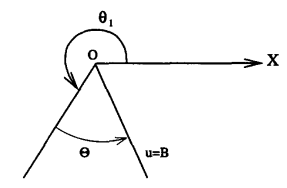
\includegraphics[scale=0.5]{Images/rotated_wedge.png}
        \caption{Rotation of the wedge domain. Image taken from \cite{li2000singularities}.}
        \label{rotated_wedge}
    \end{figure}
    In applications, we are mostly concerned with Dirichlet-Dirichlet, Dirichlet-Neumann and Neumann-Dirichlet boundary conditions. Just like stated above, some of these boundary conditions have different expansions for the angles \(\Theta=\frac{\pi}{2}\) and \(\Theta=\frac{3\pi}{2}\). However, we are only concerned with the expansion
    \[
        v(r,\theta) = \sum_{k=0}^{\infty}\alpha_k r^{\alpha_k}\psi(\alpha_k \theta)
    \]
    where \(\psi=\sin\) or \(\psi = \cos\). In these cases, if we neglect the other terms, for the special angle \(\Theta = \frac{\pi}{2}\) above we would find that \(\alpha_k \in \mathbb{N}\). Without going in dept in singularity analysis, then its partial derivative \(\partial_r v(r,\theta)\) would be of the form 
    \[
        \partial_r v(r,\theta) = \sum_{k=0}^{\infty}\alpha_k^2 r^{\alpha_k-1}\psi(\alpha_k \theta)
    \]
    where \(\alpha_k-1 \in \mathbb{N}\). In general, if \(\alpha_k \in \mathbb{N}\) for some angle \(\Theta\) then all of its derivatives are continuous and \(v(r,\theta)\) is analytical. More precisely, there is no singularity in these cases. Therefore, one does not need to enrich the set of basis functions since the fundamental solutions correctly reproduce the behavior near the corner's tip. Such corners are called \textit{regular}. On the other hand, corners which present singularities are called \textit{singular} and are the ones which we are interested to better approximate. 

    Also notice that, in the expansions above, the term \(r^{-\alpha_k}\) does not appear. This has to do with the fact we are dealing with an interior problem: when considering the exterior problem, the terms \(r^{\alpha_k}\) are replaced with \(r^{-\alpha_k}\) (observe that it satisfies the asymptotic conditions prescribed in order to have well-posedness!).
\end{remark}

To incorporate the singular behavior near a singular corner, first assume, without loss of generality, that the domain \(\Omega\) has just one corner and that the solution of our BVP can be decomposed in regular and singular parts,
\[
    u(x) = u_R(x) + u_S(x), \; x \in \overline{\Omega},
\]
where \(u_R\) is the regular part is approximated by the MFS basis functions, and the singular part \(u_S\) is approximated by the expansions above, having the boundary conditions into account. Let \(\phi_s(r, \theta)\) be one of those expansions centered at the corner's tip, where \(s\) is the order of the expansion. Then, the numerical approximation can be written as
\begin{equation}
    \tilde{u}(x) = \sum_{j=1}^{N}\alpha_j \Phi(x-y_j) + \alpha_{N+1} + \sum_{s=1}^{p} \beta_s \phi_s(r(x),\theta(x)), \; x \in \overline{\Omega}.
\end{equation}
Considering the collocation points \(x_1,\dots,x_M \in \partial \Omega\), the linear system of equations \eqref{mfs_m_system} can be generalized to
\begin{equation}
    {\underbrace{\bigg[ \begin{array}{c | c}
        A_1 & B_1 \\
    \end{array} \bigg]}_{A}}_{M\times(N+1+P)}
    \begin{bmatrix}
        \alpha\\
        \beta
    \end{bmatrix}_{(N+1+P)\times 1}
    =
    \bigg[ \begin{array}{c}
        g \\
    \end{array} \bigg]_{M\times 1},
\end{equation}
where the block matrix \(A_1\) is the matrix \(A\) in \eqref{mfs_m_system} and the \(B_1\) block matrix is given by
\[
    B_1=\begin{bmatrix}
        \phi_1(r(x_1), \theta(x_1)) & \cdots & \phi_p(r(x_1), \theta(x_1)) \\
        \vdots & \ddots & \vdots\\
        \phi_1(r(x_M), \theta(x_M)) & \cdots & \phi_p(r(x_M), \theta(x_M)).
    \end{bmatrix}
\]


\section{Numerical approach for the Helmholtz Equation}
For the Helmholtz equation, the MFS convergence and stability results resemble the previous ones for the Laplace equation with Dirichlet boundary conditions. Once again, the results are stated for identical geometries as before, where \(\Omega\) is the unit disk and the radius of \(\hat{\Omega}\) is \(R>1\). Here is assumed that the boundary data \(g\) can be analytically extended to the annulus \(\{z \in \mathbb{C}: \frac{1}{\rho}< \abs{z} < \rho\}\), where \(\rho > 1\). The following result is due to \cite{barnett2008stability}.
\begin{theorem}
    Let \(R > 1\) and \(N\) be an even number. Then the minimum boundary error achieved by the MFS in the unit disk satisfies
    \[
        \norm{g - \tilde{u}_{|\Gamma}}_{L^2(\Gamma)} \leq 
        \begin{cases}
            C \rho^{-\frac{N}{2}}, \text{ if } \rho < R^2\\
            C \sqrt{N} R^{-N}, \text{ if } \rho = R^2\\
            C R^{-N}, \text{ if } \rho > R^2\\
        \end{cases}
    \]
    where \(C\) is a constant that not depends on \(N\).
\end{theorem}
To solve the Helmholtz equation with the MFS, one must start by computing the eigenvalues \(\lambda\) (or the eigenfrequencies \(k\), with \(\lambda = k^2\)) first. In order to achieve that, recall that the Helmholtz equation
\[
    \begin{cases}
        -\Delta u = \lambda u, \text{ in } \Omega\\
        u = 0, \text{ on } \partial \Omega
    \end{cases}
\]
is well-posed when \(\lambda\) is not an eigenvalue, and in that case the nullspace of the single layer potential operator
\[
    S_k \varphi(y) = \int_{\hat{\Gamma}} \Phi_k(x-y)\varphi(x) d\sigma(x) 
\]
is trivial. More precisely, one can prove the following result, e.g. \cite{alves2005method}.
\begin{theorem}\label{mfs_helm_null_kern}
    If \(k\) is not an eigenfrequency of the interior Dirichlet problem, then \(\dim \left(N(S_k)\right)=0\).
\end{theorem}
\begin{proof}
    If \(k\) is not an eigenfrequency, then the interior problem is well posed which implies that \(\varphi(x) = 0, \; x \in \overline{\Omega}\). By analytical continuation, \(\varphi(x) = 0, \; x \in \hat{\Omega}\). Since the single layer potential is continuous, then \(\varphi(x) = 0, \; x \in \hat{\Gamma}\). By the well-posedness of the exterior problem (notice that the single layer potential satisfies the Sommerfeld radiation conditions), then \(\varphi(x) = 0, \; \forall x \in \mathbb{R}^2\).
\end{proof}

This theorem can be used to search for the eigenvalues/eigenfrequencies of the Laplace operator. By virtue of the discretization of the single layer potential \eqref{mfs_approx_disc}, one should find the values \(k\) such that the nullspace of the matrix \(A(k) = \begin{bmatrix}
    \Phi_k(x_i - y_j)
\end{bmatrix}_{M \times N}\) is not trivial. Like it was discussed in the previous section \ref{n_a_mfs_lap}, that can be done in two different ways:
\begin{enumerate}
    \item if \(A(k)\) is a square matrix (with \(M=N\)), one can compute the determinant of \(A(k)\). Since the components of \(A(k)\) are complex numbers, then its determinant is also a complex number, and we consider its absolute value. In any case, instead of working with \(\abs{\determinant A(k)}\), since this value is very small, one must work with its logarithm and consider the function \(d(k) = \log \abs{\determinant A(k)}\);
    \item if \(A(k)\) is an \(M\times N\) rectangular matrix, with \(M > N\), one considers the smallest singular value, which we denote by \(\sigma_N(k)\), where the singular values of \(A(k)\) are assumed to be in decreasing order \(\sigma_1(k) \geq \dots \geq \sigma_N(k)\). We emphasize that we only work with this case.
\end{enumerate}
Therefore, in order to find the eigenvalues/eigenfrequencies of the Laplace operator, one must find the singularities of the functions \(d(k)\) or \(\sigma_N(k)\) for the first and second cases above, respectively.

\subsection{The Subspace Angle Technique}

Again, one of the drawbacks of this method is the ill-conditioning of the system. In this subsection we introduce the so-called \textit{Subspace Angle Technique}, first presented in \cite{betcke2005reviving}. Intuitively, there are two problems at play: firstly, while the MFS only needs the boundary data to approximate the solution of the BVP, the exponential growth of the condition number against the exponential convergence can be seen has the lack of information given by the collocation points on the boundary, which is not enough to decide if an approximate eigenfunction is spurious; secondly, while we proved the linear independence of the basis functions, in practice the columns of the matrix \(A(k)\) are almost linear dependent if its number is too large (in fact, this is, once again, associated with the distance from the boundary to the artificial boundary).

To solve the first problem, we add additional interior points in order to over determine the system; and for the second problem we construct an orthonormal basis of the column space of \(A(k)\), denoted by \(\mathcal{C}(A(k))\), using the \(QR\) factorization of \(A(k)\). Let \(M_B\) be the number of boundary points and \(M_I\) the number of interior points, such that \(M=M_B+M_I\). Then, by adding some interior points the matrix \(A(k)\) can be extended to
\[
    A(k) = \begin{bmatrix}
        A_B(k)\\
        A_I(k)
    \end{bmatrix},
\]
where the indices \(B\) and \(I\) correspond to the block matrices with the boundary and interior collocation points, respectively. To generate an orthonormal basis of the column space of \(A(k)\), consider the \(QR\) factorization of \(A(k)\), given by \(A(k)=Q(k)R\), where \(Q(k)\) is a unitary complex matrix (i.e., \(Q^\dagger(k) = Q^{-1}(k)\)) and \(R\) is an upper triangular matrix. By partitioning \(Q(k)\) in the boundary and interior collocation points we also have
\begin{equation*}
    Q(k) = \begin{bmatrix}
        Q_B(k)\\
        Q_I(k)
    \end{bmatrix},
\end{equation*}
and each unit vector \(u \in \mathcal{C}(A(k))\) has the form
\begin{equation}\label{sat_qr}
    u = \begin{bmatrix}
        u_B\\
        u_I
    \end{bmatrix} = Q(k)v = \begin{bmatrix}
        Q_B(k)\\
        Q_I(k)
    \end{bmatrix}v
\end{equation}
for some \(v \in \mathbb{R}^2\), \(\norm*{v} = 1\). Assuming homogeneous Dirichlet boundary conditions, we are interested in non-trivial solutions \(v \in \mathbb{R}^2\) to the above problem when \(u \approx 0\) at the boundary, i.e, to solve the constrained minimization problem
\[
    \min_{v \in \mathbb{R}^2, \norm*{v}=1} \norm*{Q_B(k) v}. 
\]
The above problem is easy to solve and has a closed form solution which can be found using Lagrange multipliers. The solution \(\check{v}\) is the right singular vector associated with the smallest singular value \(\sigma_N\) and
\[
    \sigma_N(k) = \norm*{Q_B(k) \check{v}}.
\]
Let \(\check{u} = Q(k) \check{v}\). Taking the norm on both sides of equation \eqref{sat_qr}, one can write
\begin{equation}\label{sat_eq}
    1 = \norm{\check{u}}^2 = \norm{\begin{bmatrix}
        Q_B(k)\\
        Q_I(k)
    \end{bmatrix}\check{v}}^2 = \sigma_N^2(k) + \norm*{Q_I(k) \check{v}}^2.
\end{equation}
Notice how equation \eqref{sat_eq} can be used to eliminate spurious solutions: since \(0 < \sigma_N < 1\), if \(\sigma_N \approx 1\), then \(Q_I(k) \check{v} \approx 0 \implies u_I \approx 0\) which is an incorrect solution (is zero on the interior and does not satisfy the boundary constraints); on the other hand, if \(\sigma_N \approx 0\), then we found an eigenfunction which is small on the boundary points and whose interior is not null.

The name Subspace Angle Technique comes from the fact that \(\sigma_N\) is related with the angle between the subspaces \(\mathcal{C}(A(k))\) and \(\mathcal{G}_0\), the space of vectors that are zero at boundary points\footnote{\(\mathcal{G}_0\) can be seen as the discretization of the functions which satisfy the boundary conditions but not the Helmholtz equation.}. The angle \(\phi(k)=\angle (\mathcal{C}(A(k)), \mathcal{G}_0)\) between both subspaces is defined by
\[
    \cos \phi(k) = \sup_{\substack{u \in \mathcal{C}(A(k)), \, \norm{u}=1 \\ v \in \mathcal{G}_0, \, \norm*{v} = 1}} (u, v),
\]
and one can prove (c.f. \cite{betcke2005reviving}) that
\[
    \sigma_N = \sin \phi(k).
\]
Therefore, the discrete problem has a non-trivial solution (i.e. \(\lambda\) is an eigenvalue of the Laplace Operator) if and only if \(\mathcal{C}(A(k))\) and \(\mathcal{G}_0\) have a non-trivial intersection (i.e. \(\phi(k) = l \pi, \, l \in \mathbb{Z}\)).

\begin{remark}
    While the construction above assumed homogeneous Dirichlet boundary conditions, it can be easily generalized to any type of homogeneous boundary conditions \(\mathcal{B}\) by considering the appropriate \(A\) matrix.
\end{remark}

\begin{remark}
    Neither the enrichment technique nor the Subspace Angle Technique are specific methods only applicable to the Laplace equation and the Helmholtz equation, respectively. They can be used for both equations and at the same time. For example, in \cite{antunes2010meshfree}, both methods were used to study the spectrum of the Laplace operator in domains with corners and cracks.
\end{remark}
